     %%%%%%%%%%%%%%%%%%%%
     %                  %
     %  capitolo1.tex   %
     %                  %
     %%%%%%%%%%%%%%%%%%%%

\section{Sviluppo dell'applicativo}

\subsection{Obiettivi}
L' obiettivo del software è quello di realizzare un applicativo che esegua model based tracking sulla base di un video passatogli come ingresso. Più nel dettaglio l'applicazione esegue il tracciamento tramite il filtro di Kalman e Condensation, in maniera tale da poter confrontare le prestazioni dell' uno e dell'altro.\\
Altri requisiti funzionali sono quelli di:

\begin{itemize}
 \item  fare scegliere all'utente l'oggetto da tracciare in caso di tracking multiplo: in questo caso il software si ferma sul primo frame del video, dando possibilità di scegliere l'oggetto di cui si vuol fare il tracciamento. Per migliorare la selezione di un oggetto, vengono evidenziati da un puntini gialli. Vedi figura \ref{fig:scelta2blob}

\item tracciare a video l'andamento dei due algoritmi, evidenziandoli con colori differenti; visualizzare un' ellissi per ogni algoritmo che indichi la varianza del vettore di stato per quel tipo di tracking.

\item fornire un output razionalizzato su terminale e su filesystem per verificare rispettivamente la corretta esecuzione degli algoritmi e per avere un riscontro finale sulle performance e l'accuratezza di ognuno. Successivamente parsare i suddetti file per una rappresentazione grafica dell'accuratezza dei due metodi di tracking.

\item progettare e realizzare l'applicazione in maniera tale che possa essere compilata ed eseguite su piattaforme diverse.


\end{itemize}

\begin{figure}[hb]
\centering
	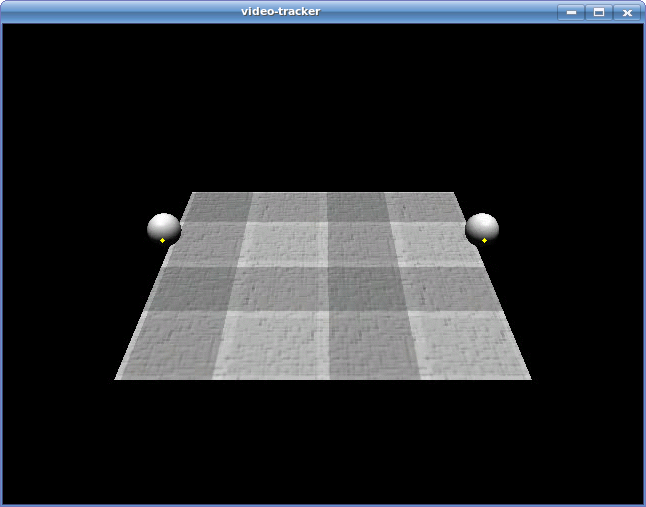
\includegraphics[scale=0.5]{doppiascelta.png}
\caption[Esempio di scelta tra due blob]{\textit{Esempio di scelta tra due blob su tracking multiplo: l'utente ha la possibilità di sccegliere su quale blob effettuare il tracciamento semplicemente cliccando vicino ad uno dei punti gialli. Il Sistema automaticamente selezionerà il blob più vicino.}\label{fig:scelta2blob}}
\end{figure}


\'E bene sottolineare che il video in ingresso possiede delle restrizioni: infatti affinchè il background subtraction lavori in maniera ottima, è necessario che il video:
\begin{itemize}
 \item possieda semper uno sfondo fisso o che comunque non vari durante la ripresa. Cambiare sfondo sarrebbe come rinizializzare l'agoritmo per il detecting dei blob.
\item possieda un numero ( $n > 25 $ ) di frame inziale che mostrino solo il backgroundper facilitare il calcolo della \textit{ground truth}, cioè del blob osservato da cui prendere le misure per i due algoritmi.
\item sia stato registrato da una postazione fissa e che la telecamera di ripersa non introduca nel video un moto relativo.
 \end{itemize}

Per svilluppare l'applicazione sono state utilizzate le libreria \textit{OpenCV}, emergente nel campo della \textit{computer vision}  e sviluppata da Intel sotto una licenza di tipo OpenSource, compatibile con la GNU GPL.


ingresso video fatto in un certo modo (sfondo fisso, tot frame di background iniziale, telecamera fissa)

uno o + oggetti in moto

permette di selezionare QUALE oggetto seguire, farne il tracciamento reale, ottenere le predizioni secondo k e c, e raccoglierne dati e risultati per la realizzazione di grafici

intro utilizzo librerie utilizzate intel openCV
\subsection{Librerie Intel OpenCV}
OpenCv è una libreria sviluppata da Intel e rilasciata sotto la licenza ``Intel License Agreement For Open Source Computer Vision Library''. Il motivo di questa scelta si basa sul fatto che queste librerie, sviluppate da una casamadre leader nel settore del ITC, risultato implementate secondo il modello opensource, quindi vi è possibilità di visionare e/o modifcare il codice sorgente. Inoltre un' altra potenzialità offerta è la caratteristica di essere \textit{cross-platform}: cioè possono benissimo essere compilato e usate sia sotto sistema operativo Microsft Windows che GNU/Linux. Questa caratteristica le rende molto appetibili per i requisiti di portabilià che ci eravamo prefissi di raggiungere.\\ Da notare che le librerie sono scritte in linguaggio C e non fanno uso quindi di un linguaggio orientato agli oggetti.

Le librerie si focalizzano princiaplmente su processing di tipo real-time su immagini, ma forniscono diversi metodi famosi in letteratura per la manipolazione dei video. Una panoramica generale delle librerie comprende questi aspetti della computer vision:
\begin{enumerate}
\item Human-Computer Interface (HCI)
\item Object Identification
\item Segmentation and Recognition
\item Face Recognition e Gesture Recognition
\item Motion Tracking
\end{enumerate}

Come molti progetti opensource in maturazione \footnote{La versione 1.0 ufficiale è stata rilasciata nel tardo 2006; parte del progetto è stato scritto con librerie in beta testing} è stata carente la parte che riguarda la documentazione. Nonostante la presenza di un colosso alla spalle e di una struttura basata sul modello wiki, la documentazione ufficiale in pdf e html anche se ottenibile non è stata sufficiente per colmare le lacune iniziali. Per questo motivo è stato effettuato un grosso lavoro di studio per capire il funzionamento del toolkit OpenCv, che spesso è terminato con la ricerca di documentazione in sito asiatici difficili da comprendere. Sembra infatti che siano molto gradite in Giappone queste librerie.\\
Alcuni riferimenti importanti per OpenCV:
\begin{itemize}
 \item \htmladdnormallink{Sito web ufficiale}{http://www.intel.com/technology/computing/opencv/index.htm}
\item \htmladdnormallink{Portale di wiki}{http://opencvlibrary.sourceforge.net}
\end{itemize}

 
\subsection{Control Flow del programma}
intro del ciclozzo FOR e che cosa viene fatto in ordine con l'acquisizione frame/frame del video

\subsubsection{Back subtraction}
realizzazione online del backsub, librerie eccetera
\subsubsection{Predizione}
\subsubsection{Rappresentazione della predizione}
\subsubsection{HiGui}
\subsubsection{Scripting GNUPlot}

